% =====================================================================
% Appendix E: additional results (one-column appendix).
% Floats: Fig. 5 (fig:gap; moved here from Sec. 6.4, label kept),
% Table A5 (tables/tab_conditions; three parts), Fig. A3 (fig:gap-sweep),
% Fig. A5 (fig:turn-length), Table A6 (tables/tab_ca_latency),
% Table A8 (tables/tab_failures).
% Also holds detail moved out of Sec. 6: the factorial-effect formulas, the
% second-best pipeline, tcpWER, DER without a collar, the DER caveat and the
% reference configuration of each ablation row of Table 6 (paragraph
% "Ablations", pointed to from Sec. 6.5).
% Known now: the preliminary offline TAXI L0 natural rows, the offline systems'
% batched compute, and the context timings of the single-speaker 0.6B backbone.
% Everything else is a template: pending numbers are \tbd (tables) or
% \tbdtext (text). Do not describe findings before the numbers exist.
% =====================================================================
\section{Additional Results}\label{app:results}

This appendix gives the oracle gap by timing condition and language pair (\cref{fig:gap}) with the full numbers behind it and behind \cref{tab:main} (\cref{tab:conditions}), the decomposition of the gap, a dose-response analysis over the inter-turn gap (\cref{fig:gap-sweep}), latency by source-turn duration (\cref{fig:turn-length}), computation-aware latency (\cref{tab:ca-latency}), a failure taxonomy (\cref{tab:failures}), further transcript and speaker metrics, and the variants of \cref{tab:ablation}. All analyses follow the protocol of \cref{sec:bench}: 95\% session-clustered bootstrap intervals, and no threshold or operating point tuned on TAXI. So far, only the offline rows on \taxi L0 natural (preliminary) and a few timings exist.
\draftnote{every other cell is pending; L1, the fixed-gap renders and \syn are planned}

\paragraph{Gap by timing condition and language pair.}
\Cref{fig:gap}, summarised in \cref{sec:exp-timing}, contrasts for every timing condition and language pair the reference pipeline $P$ of \cref{sec:exp-setup} under the oracle and the realistic wrapper with \model, which receives no oracle input. One pipeline serves every row and both wrappers, so that each gap compares the same system with and without oracle segmentation and routing. COMET is averaged over the two directions; as one side of every synthetic pair is translationese (\cref{app:syn}), rows are compared only through their gaps, never through absolute COMET.

\begin{figure}[t]
  \centering
  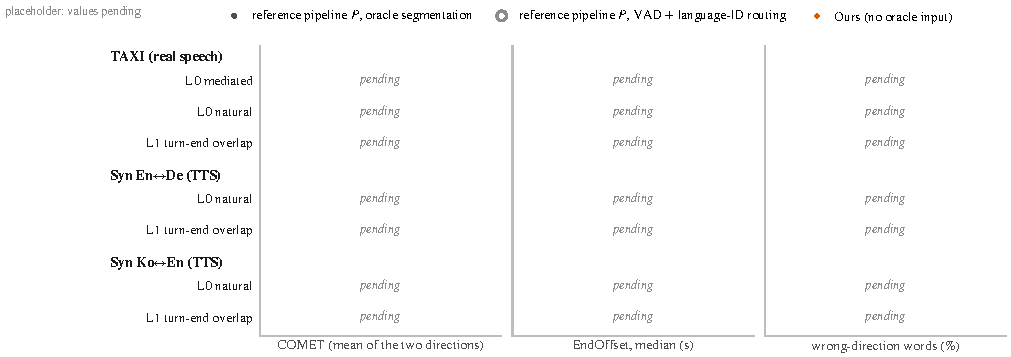
\includegraphics{figures/fig5_oracle_gap.pdf}
  \caption{Where the conversational difficulty lies (values pending; numbers will be in \cref{tab:conditions}). For each timing condition and language pair: the reference pipeline $P$ with oracle turn segmentation (filled) and with VAD and language-ID routing (hollow), and \model (diamond; no oracle input). $P$ covers both directions and has the highest realistic-wrapper COMET on \taxi L0 natural at its main operating point (\cref{sec:exp-setup}); it serves every row and both wrappers. Panels: COMET (mean of the two directions), median \eo and wrong-direction words. Rows are compared only through their gaps, not through absolute COMET.}
  \label{fig:gap}
\end{figure}

\paragraph{Full grid.}
For every timing condition, language pair and direction, \cref{tab:conditions} lists the systems run under it, each at its main operating point, fixed before the test runs; part~(a) also repeats every row of \cref{tab:main}, so that each has its interval. The offline systems receive gold turns and translate each turn after it ends. Their \laal therefore equals the mean source-turn duration (4.624\,s for \ende and 3.086\,s for \deen on \taxi), and their \eo is 0 on the ideal clock because their output is time-stamped at the gold turn end; \cref{tab:ca-latency} adds their compute. The gold-transcript row isolates translation quality, the Qwen3-ASR row adds the recognition of telephone-band speech, and Whisper ST covers \deen only. Under L1, an oracle segment cut from the mono mix also contains the overlapping speech of the other speaker; the oracle-separation row of \cref{tab:factorial} removes it. On \syn we interpret only rankings and effects relative to each pair's own offline systems with oracle input, never absolute scores across pairs.

% =====================================================================
% Table A5 (tab:conditions): full per-direction grid, the numbers behind
% Fig. 5 (fig:gap) and Fig. A3 (fig:gap-sweep). Included from App. E.
% Two floats: the second continues the first (\ContinuedFloat, caption package,
% keeps the table number; it has no label of its own).
% Known now: only the offline TAXI L0 natural rows (preliminary; the same runs
% as Table 3 / tab:main). Every other cell is pending (\tbd = blank).
% Row sets follow the experiment plan: CST-Bench-Syn runs the offline bounds,
% the three main pipelines and the model; SeamlessM4T v2 + AlignAtt runs on TAXI.
% The optional L1b stress test (not in v1) would add its own block and a
% backchannel-leakage column. When filling cells, keep the block structure.
% =====================================================================
\begin{table}[!tp]
  \caption{Full results by timing condition and language pair: the numbers behind \cref{fig:gap,fig:gap-sweep} (ideal clock; each system at its pre-registered main operating point). Part~(a) covers \taxi; parts~(b) and~(c) follow. Seg.: oracle = gold turns and source language; realistic = VAD and language-ID routing; none = the system segments the stream itself. Offline: gold$\to$LLM and ASR$\to$LLM translate the gold or the Qwen3-ASR-1.7B transcript of each turn with Qwen3.8-27B, and Whisper ST is Whisper-large-v3 translating into English; streaming cascade: streaming ASR and Qwen3.8-27B with LocalAgreement-2; M4T v2: SeamlessM4T v2 (\cref{tab:baselines}). X is German on \taxi and \syn \pair{En}{De}, and Korean on \syn \pair{Ko}{En}. Latencies are in seconds over non-empty turns: mean \laal and median \eo per direction; wrong-direction words, median switch latency and empty turns are pooled over both directions; \cref{tab:ca-latency} lists each system's encoder look-ahead $\ell_{\mathrm{enc}}$. Each estimate will carry the half-width of its 95\% session-clustered bootstrap CI as a subscript. Offline systems translate each oracle turn after it ends, so their \laal equals the mean source-turn duration and their \eo is 0 by construction. $^\dagger$preliminary; to be re-run under the final protocol (same runs as \cref{tab:main}; no CIs yet). --: not applicable; blank: pending. \protect\draftnote{L1 is not rendered yet}}
  \label{tab:conditions}
  \centering
  \footnotesize
  \setlength{\tabcolsep}{3pt}
  \begin{tabular}{@{}llccccccccccc@{}}
    \toprule
    & & \multicolumn{4}{c}{\dir{En}{X}} & \multicolumn{4}{c}{\dir{X}{En}} & \multicolumn{3}{c}{Both directions} \\
    \cmidrule(lr){3-6}\cmidrule(lr){7-10}\cmidrule(l){11-13}
    System & Seg. & COMET & chrF & \makecell{Stream-\\LAAL} & \makecell{End-\\Offset} & COMET & chrF & \makecell{Stream-\\LAAL} & \makecell{End-\\Offset} & \makecell{Wrong\\dir.\ (\%)} & \makecell{Switch\\latency} & \makecell{Empty\\turns (\%)} \\
    \midrule
    \multicolumn{13}{@{}l}{\textit{(a) \taxi, L0 natural}} \\
    Offline: gold$\to$LLM & oracle & \tbd & \prelim{71.72} & \prelim{4.62} & 0 & \tbd & \prelim{58.05} & \prelim{3.09} & 0 & \tbd & \tbd & \tbd \\
    Offline: ASR$\to$LLM & oracle & \tbd & \prelim{67.97} & \prelim{4.62} & 0 & \tbd & \prelim{56.61} & \prelim{3.09} & 0 & \tbd & \tbd & \tbd \\
    Offline: Whisper ST & oracle & -- & -- & -- & -- & \tbd & \prelim{56.67} & \prelim{3.09} & 0 & \tbd & \tbd & \tbd \\
    Consecutive cascade & realistic & \tbd & \tbd & \tbd & \tbd & \tbd & \tbd & \tbd & \tbd & \tbd & \tbd & \tbd \\
    SeamlessStreaming & oracle & \tbd & \tbd & \tbd & \tbd & \tbd & \tbd & \tbd & \tbd & \tbd & \tbd & \tbd \\
    SeamlessStreaming & realistic & \tbd & \tbd & \tbd & \tbd & \tbd & \tbd & \tbd & \tbd & \tbd & \tbd & \tbd \\
    Streaming cascade & oracle & \tbd & \tbd & \tbd & \tbd & \tbd & \tbd & \tbd & \tbd & \tbd & \tbd & \tbd \\
    Streaming cascade & realistic & \tbd & \tbd & \tbd & \tbd & \tbd & \tbd & \tbd & \tbd & \tbd & \tbd & \tbd \\
    M4T v2 + AlignAtt & oracle & \tbd & \tbd & \tbd & \tbd & \tbd & \tbd & \tbd & \tbd & \tbd & \tbd & \tbd \\
    M4T v2 + AlignAtt & realistic & \tbd & \tbd & \tbd & \tbd & \tbd & \tbd & \tbd & \tbd & \tbd & \tbd & \tbd \\
    \model & none & \tbd & \tbd & \tbd & \tbd & \tbd & \tbd & \tbd & \tbd & \tbd & \tbd & \tbd \\
    \midrule
    \multicolumn{13}{@{}l}{\textit{\taxi, L0 mediated}} \\
    Offline: gold$\to$LLM & oracle & \tbd & \tbd & \tbd & \tbd & \tbd & \tbd & \tbd & \tbd & \tbd & \tbd & \tbd \\
    Offline: ASR$\to$LLM & oracle & \tbd & \tbd & \tbd & \tbd & \tbd & \tbd & \tbd & \tbd & \tbd & \tbd & \tbd \\
    Offline: Whisper ST & oracle & -- & -- & -- & -- & \tbd & \tbd & \tbd & \tbd & \tbd & \tbd & \tbd \\
    Consecutive cascade & realistic & \tbd & \tbd & \tbd & \tbd & \tbd & \tbd & \tbd & \tbd & \tbd & \tbd & \tbd \\
    SeamlessStreaming & oracle & \tbd & \tbd & \tbd & \tbd & \tbd & \tbd & \tbd & \tbd & \tbd & \tbd & \tbd \\
    SeamlessStreaming & realistic & \tbd & \tbd & \tbd & \tbd & \tbd & \tbd & \tbd & \tbd & \tbd & \tbd & \tbd \\
    Streaming cascade & oracle & \tbd & \tbd & \tbd & \tbd & \tbd & \tbd & \tbd & \tbd & \tbd & \tbd & \tbd \\
    Streaming cascade & realistic & \tbd & \tbd & \tbd & \tbd & \tbd & \tbd & \tbd & \tbd & \tbd & \tbd & \tbd \\
    M4T v2 + AlignAtt & oracle & \tbd & \tbd & \tbd & \tbd & \tbd & \tbd & \tbd & \tbd & \tbd & \tbd & \tbd \\
    M4T v2 + AlignAtt & realistic & \tbd & \tbd & \tbd & \tbd & \tbd & \tbd & \tbd & \tbd & \tbd & \tbd & \tbd \\
    \model & none & \tbd & \tbd & \tbd & \tbd & \tbd & \tbd & \tbd & \tbd & \tbd & \tbd & \tbd \\
    \midrule
    \multicolumn{13}{@{}l}{\textit{\taxi, L1 (turn-end overlap)}} \\
    Offline: gold$\to$LLM & oracle & \tbd & \tbd & \tbd & \tbd & \tbd & \tbd & \tbd & \tbd & \tbd & \tbd & \tbd \\
    Offline: ASR$\to$LLM & oracle & \tbd & \tbd & \tbd & \tbd & \tbd & \tbd & \tbd & \tbd & \tbd & \tbd & \tbd \\
    Offline: Whisper ST & oracle & -- & -- & -- & -- & \tbd & \tbd & \tbd & \tbd & \tbd & \tbd & \tbd \\
    Consecutive cascade & realistic & \tbd & \tbd & \tbd & \tbd & \tbd & \tbd & \tbd & \tbd & \tbd & \tbd & \tbd \\
    SeamlessStreaming & oracle & \tbd & \tbd & \tbd & \tbd & \tbd & \tbd & \tbd & \tbd & \tbd & \tbd & \tbd \\
    SeamlessStreaming & realistic & \tbd & \tbd & \tbd & \tbd & \tbd & \tbd & \tbd & \tbd & \tbd & \tbd & \tbd \\
    Streaming cascade & oracle & \tbd & \tbd & \tbd & \tbd & \tbd & \tbd & \tbd & \tbd & \tbd & \tbd & \tbd \\
    Streaming cascade & realistic & \tbd & \tbd & \tbd & \tbd & \tbd & \tbd & \tbd & \tbd & \tbd & \tbd & \tbd \\
    M4T v2 + AlignAtt & oracle & \tbd & \tbd & \tbd & \tbd & \tbd & \tbd & \tbd & \tbd & \tbd & \tbd & \tbd \\
    M4T v2 + AlignAtt & realistic & \tbd & \tbd & \tbd & \tbd & \tbd & \tbd & \tbd & \tbd & \tbd & \tbd & \tbd \\
    \model & none & \tbd & \tbd & \tbd & \tbd & \tbd & \tbd & \tbd & \tbd & \tbd & \tbd & \tbd \\
    \bottomrule
  \end{tabular}
\end{table}

\begin{table}[!tp]
  \ContinuedFloat
  \caption[]{(continued) Part~(b): \syn, with the columns and conventions of part~(a). Part~(c): \taxi re-rendered with one fixed gap at every speaker change (a negative gap starts the next turn before the previous one ends), the numbers behind \cref{fig:gap-sweep}; COMET is the mean of the two directions, \eo the median over both directions, and the best pipeline is that of \cref{tab:factorial}. If the optional L1b stress test is adopted, it adds a block with a backchannel-leakage column. Blank: pending. \protect\draftnote{\syn and the fixed-gap renders are planned}}
  \centering
  \footnotesize
  \setlength{\tabcolsep}{3pt}
  \begin{tabular}{@{}llccccccccccc@{}}
    \toprule
    & & \multicolumn{4}{c}{\dir{En}{X}} & \multicolumn{4}{c}{\dir{X}{En}} & \multicolumn{3}{c}{Both directions} \\
    \cmidrule(lr){3-6}\cmidrule(lr){7-10}\cmidrule(l){11-13}
    System & Seg. & COMET & chrF & \makecell{Stream-\\LAAL} & \makecell{End-\\Offset} & COMET & chrF & \makecell{Stream-\\LAAL} & \makecell{End-\\Offset} & \makecell{Wrong\\dir.\ (\%)} & \makecell{Switch\\latency} & \makecell{Empty\\turns (\%)} \\
    \midrule
    \multicolumn{13}{@{}l}{\textit{(b) \syn \pair{En}{De}, L0 natural}} \\
    Offline: gold$\to$LLM & oracle & \tbd & \tbd & \tbd & \tbd & \tbd & \tbd & \tbd & \tbd & \tbd & \tbd & \tbd \\
    Offline: ASR$\to$LLM & oracle & \tbd & \tbd & \tbd & \tbd & \tbd & \tbd & \tbd & \tbd & \tbd & \tbd & \tbd \\
    Consecutive cascade & realistic & \tbd & \tbd & \tbd & \tbd & \tbd & \tbd & \tbd & \tbd & \tbd & \tbd & \tbd \\
    SeamlessStreaming & oracle & \tbd & \tbd & \tbd & \tbd & \tbd & \tbd & \tbd & \tbd & \tbd & \tbd & \tbd \\
    SeamlessStreaming & realistic & \tbd & \tbd & \tbd & \tbd & \tbd & \tbd & \tbd & \tbd & \tbd & \tbd & \tbd \\
    Streaming cascade & oracle & \tbd & \tbd & \tbd & \tbd & \tbd & \tbd & \tbd & \tbd & \tbd & \tbd & \tbd \\
    Streaming cascade & realistic & \tbd & \tbd & \tbd & \tbd & \tbd & \tbd & \tbd & \tbd & \tbd & \tbd & \tbd \\
    \model & none & \tbd & \tbd & \tbd & \tbd & \tbd & \tbd & \tbd & \tbd & \tbd & \tbd & \tbd \\
    \midrule
    \multicolumn{13}{@{}l}{\textit{\syn \pair{En}{De}, L1 (turn-end overlap)}} \\
    Offline: gold$\to$LLM & oracle & \tbd & \tbd & \tbd & \tbd & \tbd & \tbd & \tbd & \tbd & \tbd & \tbd & \tbd \\
    Offline: ASR$\to$LLM & oracle & \tbd & \tbd & \tbd & \tbd & \tbd & \tbd & \tbd & \tbd & \tbd & \tbd & \tbd \\
    Consecutive cascade & realistic & \tbd & \tbd & \tbd & \tbd & \tbd & \tbd & \tbd & \tbd & \tbd & \tbd & \tbd \\
    SeamlessStreaming & oracle & \tbd & \tbd & \tbd & \tbd & \tbd & \tbd & \tbd & \tbd & \tbd & \tbd & \tbd \\
    SeamlessStreaming & realistic & \tbd & \tbd & \tbd & \tbd & \tbd & \tbd & \tbd & \tbd & \tbd & \tbd & \tbd \\
    Streaming cascade & oracle & \tbd & \tbd & \tbd & \tbd & \tbd & \tbd & \tbd & \tbd & \tbd & \tbd & \tbd \\
    Streaming cascade & realistic & \tbd & \tbd & \tbd & \tbd & \tbd & \tbd & \tbd & \tbd & \tbd & \tbd & \tbd \\
    \model & none & \tbd & \tbd & \tbd & \tbd & \tbd & \tbd & \tbd & \tbd & \tbd & \tbd & \tbd \\
    \midrule
    \multicolumn{13}{@{}l}{\textit{\syn \pair{Ko}{En}, L0 natural}} \\
    Offline: gold$\to$LLM & oracle & \tbd & \tbd & \tbd & \tbd & \tbd & \tbd & \tbd & \tbd & \tbd & \tbd & \tbd \\
    Offline: ASR$\to$LLM & oracle & \tbd & \tbd & \tbd & \tbd & \tbd & \tbd & \tbd & \tbd & \tbd & \tbd & \tbd \\
    Consecutive cascade & realistic & \tbd & \tbd & \tbd & \tbd & \tbd & \tbd & \tbd & \tbd & \tbd & \tbd & \tbd \\
    SeamlessStreaming & oracle & \tbd & \tbd & \tbd & \tbd & \tbd & \tbd & \tbd & \tbd & \tbd & \tbd & \tbd \\
    SeamlessStreaming & realistic & \tbd & \tbd & \tbd & \tbd & \tbd & \tbd & \tbd & \tbd & \tbd & \tbd & \tbd \\
    Streaming cascade & oracle & \tbd & \tbd & \tbd & \tbd & \tbd & \tbd & \tbd & \tbd & \tbd & \tbd & \tbd \\
    Streaming cascade & realistic & \tbd & \tbd & \tbd & \tbd & \tbd & \tbd & \tbd & \tbd & \tbd & \tbd & \tbd \\
    \model & none & \tbd & \tbd & \tbd & \tbd & \tbd & \tbd & \tbd & \tbd & \tbd & \tbd & \tbd \\
    \midrule
    \multicolumn{13}{@{}l}{\textit{\syn \pair{Ko}{En}, L1 (turn-end overlap)}} \\
    Offline: gold$\to$LLM & oracle & \tbd & \tbd & \tbd & \tbd & \tbd & \tbd & \tbd & \tbd & \tbd & \tbd & \tbd \\
    Offline: ASR$\to$LLM & oracle & \tbd & \tbd & \tbd & \tbd & \tbd & \tbd & \tbd & \tbd & \tbd & \tbd & \tbd \\
    Consecutive cascade & realistic & \tbd & \tbd & \tbd & \tbd & \tbd & \tbd & \tbd & \tbd & \tbd & \tbd & \tbd \\
    SeamlessStreaming & oracle & \tbd & \tbd & \tbd & \tbd & \tbd & \tbd & \tbd & \tbd & \tbd & \tbd & \tbd \\
    SeamlessStreaming & realistic & \tbd & \tbd & \tbd & \tbd & \tbd & \tbd & \tbd & \tbd & \tbd & \tbd & \tbd \\
    Streaming cascade & oracle & \tbd & \tbd & \tbd & \tbd & \tbd & \tbd & \tbd & \tbd & \tbd & \tbd & \tbd \\
    Streaming cascade & realistic & \tbd & \tbd & \tbd & \tbd & \tbd & \tbd & \tbd & \tbd & \tbd & \tbd & \tbd \\
    \model & none & \tbd & \tbd & \tbd & \tbd & \tbd & \tbd & \tbd & \tbd & \tbd & \tbd & \tbd \\
    \bottomrule
  \end{tabular}

  \vspace{1.2em}
  \begin{tabular}{@{}lccccccccc@{}}
    \toprule
    & \multicolumn{3}{c}{Best pipeline, oracle} & \multicolumn{3}{c}{Best pipeline, realistic} & \multicolumn{3}{c}{\model} \\
    \cmidrule(lr){2-4}\cmidrule(lr){5-7}\cmidrule(l){8-10}
    Gap (s) & COMET & \makecell{Wrong\\dir.\ (\%)} & \makecell{End-\\Offset (s)} & COMET & \makecell{Wrong\\dir.\ (\%)} & \makecell{End-\\Offset (s)} & COMET & \makecell{Wrong\\dir.\ (\%)} & \makecell{End-\\Offset (s)} \\
    \midrule
    \multicolumn{10}{@{}l}{\textit{(c) \taxi, one fixed gap at every speaker change}} \\
    $-0.6$ & \tbd & \tbd & \tbd & \tbd & \tbd & \tbd & \tbd & \tbd & \tbd \\
    $-0.4$ & \tbd & \tbd & \tbd & \tbd & \tbd & \tbd & \tbd & \tbd & \tbd \\
    $-0.2$ & \tbd & \tbd & \tbd & \tbd & \tbd & \tbd & \tbd & \tbd & \tbd \\
    $0.05$ & \tbd & \tbd & \tbd & \tbd & \tbd & \tbd & \tbd & \tbd & \tbd \\
    $0.2$ & \tbd & \tbd & \tbd & \tbd & \tbd & \tbd & \tbd & \tbd & \tbd \\
    $0.5$ & \tbd & \tbd & \tbd & \tbd & \tbd & \tbd & \tbd & \tbd & \tbd \\
    $1.0$ & \tbd & \tbd & \tbd & \tbd & \tbd & \tbd & \tbd & \tbd & \tbd \\
    $2.0$ & \tbd & \tbd & \tbd & \tbd & \tbd & \tbd & \tbd & \tbd & \tbd \\
    \bottomrule
  \end{tabular}
\end{table}


\paragraph{Decomposing the gap.}
Let $Q_{TL}$ be the COMET of the row of \cref{tab:factorial} with gold turns ($T{=}1$) or VAD segments ($T{=}0$) and with the gold ($L{=}1$) or the identified ($L{=}0$) source language, so that the oracle gap of \cref{sec:exp-setup} is $G=Q_{11}-Q_{00}$. The segmentation effect
\begin{equation*}
  E_T=\tfrac12\bigl[(Q_{11}-Q_{01})+(Q_{10}-Q_{00})\bigr]
\end{equation*}
and the routing effect $E_L=\tfrac12[(Q_{11}-Q_{10})+(Q_{01}-Q_{00})]$ each average the loss from replacing one oracle component over both settings of the other component. They sum to $G$, which makes them the Shapley attribution for two factors, and the interaction $I=Q_{11}-Q_{10}-Q_{01}+Q_{00}$ measures how far the two losses compound. We report $E_T$, $E_L$ and $I$ in COMET points with session-bootstrap CIs, not as shares of $G$, which are unstable when $G$ is small. Repeating the factorial for the second-best pipeline (\tbdtext{}) gives $E_T$ and $E_L$ of \tbdtext{} and \tbdtext{} COMET under L1.

\paragraph{Gap dose-response.}
Each timing condition draws its gaps from one distribution. To test whether pipelines degrade smoothly as turns follow each other more closely, we re-render \taxi with one fixed gap $g$ at every speaker change, $g\in\{-0.6,-0.4,-0.2,0.05,0.2,0.5,1.0,2.0\}$\,s, each rendering under its own configuration name and checksums; a negative gap starts the next turn $|g|$ before the previous one ends, as in L1. We run $P$ with both wrappers, and \model (\cref{fig:gap-sweep}; numbers in part~(c) of \cref{tab:conditions}). A smooth trend would show that the conclusions do not hinge on the chosen L0 and L1 distributions; a sharp drop would locate the gap at which VAD-based routing breaks down. From $g=2$\,s to $g=-0.6$\,s, COMET changes by \tbdtext{} with the realistic wrapper, by \tbdtext{} with oracle segmentation and by \tbdtext{} for \model.

\begin{figure}[t]
  \centering
  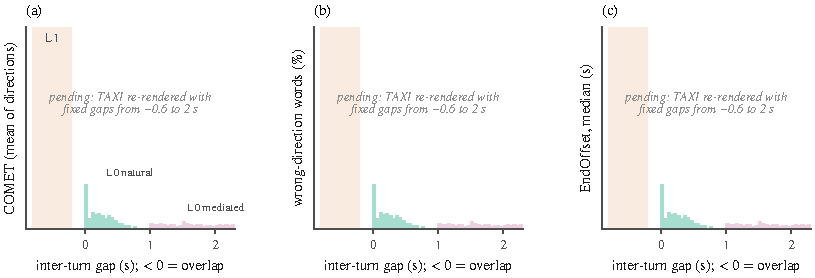
\includegraphics{figures/figA3_gap_sweep.pdf}
  \caption{Gap dose-response: \taxi re-rendered with one fixed gap at every speaker change, from $-0.6$\,s (overlap) to 2\,s. (a)~COMET (mean of the two directions), (b)~wrong-direction words and (c)~median \eo for the reference pipeline $P$ (solid: oracle segmentation; dashed: VAD and language-ID routing) and \model. Background histograms show the gaps drawn at the 540 speaker changes under L0 natural (green) and L0 mediated (pink); the shaded band is the overlap range of L1, whose next turn starts 0.2--0.8\,s before the previous one ends. Numbers in part~(c) of \cref{tab:conditions}. \protect\draftnote{results pending; the fixed-gap renders are planned}}
  \label{fig:gap-sweep}
\end{figure}

\paragraph{Why simultaneous? Latency by turn length.}
With oracle endpoints, offline systems reach an \eo of 0 on the ideal clock, which raises the question of why simultaneity is needed at all. A deployed consecutive system must first detect that a turn has ended, so the listener waits for the endpoint detector and, on the computation-aware clock, also for the translation of the whole turn. Lag within a turn grows with the turn as well: a system that emits a turn's translation only after the turn ends scores a \laal of at least the turn's duration (\cref{sec:bench}). \taxi turns are short (median 2.86\,s), but 22.5\% of them exceed 5\,s (\cref{tab:taxi-full}). \Cref{fig:turn-length} therefore breaks median \eo and \laal down by source-turn duration for the realistic consecutive cascade, the best realistic streaming pipeline and \model. For turns longer than 6\,s, the median \eo is \tbdtext{}\,s for the consecutive cascade, \tbdtext{}\,s for the best streaming pipeline and \tbdtext{}\,s for \model.

\begin{figure}[t]
  \centering
  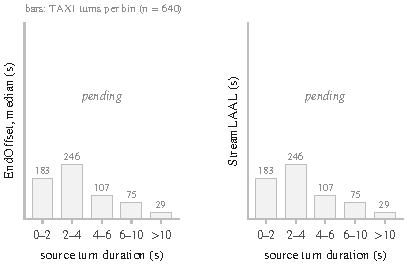
\includegraphics{figures/figA5_turn_length.pdf}
  \caption{Why simultaneous? Median \eo (left) and \laal (right) by source-turn duration on \taxi L0 natural, for the realistic consecutive cascade, the best realistic streaming pipeline and \model. Bars: \taxi turns per duration bin (183, 246, 107, 75 and 29 of 640). \protect\draftnote{results pending}}
  \label{fig:turn-length}
\end{figure}

\paragraph{Computation-aware latency.}
Main-text latencies use the ideal clock. \Cref{tab:ca-latency} times every system on one H200 GPU, as a single stream without batching, and re-scores it on the computation-aware clock, on which an emission time also counts the processing time spent until the emission \citep{ma2020simulmt}. It includes the three controls of \cref{tab:ablation}, because the ideal clock hides how much their compute differs from \model's: the same-backbone cascade, for instance, re-translates the growing transcript with a 27B LLM after every update. Streaming systems receive the audio in 80\,ms chunks; we report the median and the 99th percentile of the processing time per chunk (tick) and the real-time factor (RTF). Consecutive and offline systems are timed per turn. The only timings so far were taken outside this protocol. The single-speaker backbone with the 0.6B thinker takes about 60\,ms per chunk at the median on an H200 but 100--150\,ms at the 99th percentile, so it misses the 80\,ms budget there; on an M4 Mac with the thinker in MLX (fp16), it takes 56\,ms per chunk at the median and runs at an RTF of 0.82. In the preliminary offline run, batched compute moved the median \eo of the offline systems from 0 to at most about \prelim{0.2}\,s ($^\dagger$preliminary; to be re-run under the final protocol). The 1.7B thinker has not been timed, and we claim real time only for a system with a measured RTF below 1.

% =====================================================================
% Table A6 (tab:ca-latency): computation-aware latency and real-time factor.
% Included from App. E. Referenced from Secs. 4, 5, 6 and 7.
% Known now: (i) context rows = earlier measurements of the single-speaker
% 0.6B backbone (H200: tick p50 about 60 ms, p99 100-150 ms; M4 Mac with an
% MLX fp16 thinker: 56 ms p50, RTF 0.82), taken outside this protocol;
% (ii) the EndOffset of the three offline systems with measured, batched
% compute from the preliminary offline run: at most about 0.2 s (gold/ASR ->
% LLM 0.1-0.2 s, Whisper ST lower; approximate; quoted only as "<= 0.2");
% (iii) values that hold by construction (offline EndOffset 0 on the ideal
% clock; l_enc = 80 ms, the bound of the [56,0] encoder, also for M1-based
% controls). The 1.7B thinker has not been timed. The controls of Table 6
% (tab:ablation) are listed because their compute differs most from the
% model's. Everything else is pending (\tbd = blank).
% =====================================================================
\begin{table}[t]
  \caption{Computation-aware latency and real-time factor (RTF) on one H200 GPU, single stream, no batching; \taxi L0 natural, pooled over both directions. $\ell_{\mathrm{enc}}$: encoder look-ahead, counted at its bound. Tick: processing time per 80\,ms input chunk; RTF: processing time over audio duration. A real-time claim needs a measured RTF below 1; a tick above 80\,ms means that the output falls behind the input for a while. Ideal clock: an emission time is the audio consumed; computation-aware (CA) clock: it also counts the processing time spent until the emission \citep{ma2020simulmt}. \laal is a mean and \eo a median over non-empty turns. The batched offline row covers the three offline systems of the preliminary offline run, with approximate compute; the context rows are earlier measurements of the single-speaker backbone with the 0.6B thinker (not a \task system), taken outside this protocol. $^\dagger$preliminary; to be re-run under the final protocol. --: not applicable or not reported; blank: pending. \protect\draftnote{planned except the batched offline row and the context rows}}
  \label{tab:ca-latency}
  \centering
  \footnotesize
  \setlength{\tabcolsep}{4pt}
  \begin{tabular}{@{}llcccccccc@{}}
    \toprule
    & & & \multicolumn{2}{c}{Tick (ms)} & & \multicolumn{2}{c}{\laal (s)} & \multicolumn{2}{c}{\eo (s)} \\
    \cmidrule(lr){4-5}\cmidrule(lr){7-8}\cmidrule(l){9-10}
    System & Hardware & $\ell_{\mathrm{enc}}$ (ms) & p50 & p99 & RTF & ideal & CA & ideal & CA \\
    \midrule
    \model (1.7B thinker)              & H200 & 80   & \tbd & \tbd & \tbd & \tbd & \tbd & \tbd & \tbd \\
    SeamlessStreaming                  & H200 & \tbd & \tbd & \tbd & \tbd & \tbd & \tbd & \tbd & \tbd \\
    Streaming cascade                  & H200 & \tbd & \tbd & \tbd & \tbd & \tbd & \tbd & \tbd & \tbd \\
    M4T v2 + AlignAtt                  & H200 & \tbd & \tbd & \tbd & \tbd & \tbd & \tbd & \tbd & \tbd \\
    Consecutive cascade (unbatched)    & H200 & --   & --   & --   & \tbd & \tbd & \tbd & \tbd & \tbd \\
    Offline: ASR$\to$LLM, per turn (unbatched) & H200 & -- & -- & -- & \tbd & \tbd & \tbd & 0 & \tbd \\
    Offline systems, batched           & --   & --   & --   & --   & --   & --   & --   & 0 & $\leq$\prelim{0.2} \\
    \midrule
    \multicolumn{10}{@{}l}{\textit{Controls of \cref{tab:ablation}}} \\
    Decoupled twin                     & H200 & 80   & \tbd & \tbd & \tbd & \tbd & \tbd & \tbd & \tbd \\
    Same-backbone cascade (M1$\to$LLM) & H200 & 80   & \tbd & \tbd & \tbd & \tbd & \tbd & \tbd & \tbd \\
    Size-matched cascade (ASR$\to$1.7B LLM) & H200 & \tbd & \tbd & \tbd & \tbd & \tbd & \tbd & \tbd & \tbd \\
    \midrule
    \multicolumn{10}{@{}l}{\textit{Context: single-speaker ASR backbone, 0.6B thinker (not a \task system)}} \\
    0.6B backbone                      & H200   & 80 & $\approx$60 & 100--150 & --   & -- & -- & -- & -- \\
    0.6B backbone, MLX fp16 thinker    & M4 Mac & 80 & 56          & --       & 0.82 & -- & -- & -- & -- \\
    \bottomrule
  \end{tabular}
\end{table}


\paragraph{Failure taxonomy.}
\Cref{tab:failures} counts six failure types per 100 source turns; short turns are a particular risk, as 59 \taxi turns have at most three words. The detectors work on the scorer's alignments and timelines, so the table reports counts without showing any TAXI text, and their thresholds are fixed before the test runs. Merged turns, in which one VAD segment or output piece spans turns of both speakers, send one speaker's words to the wrong channel or delay the switch. A truncated tail leaves the last words of a turn untranslated, for example when a segment is closed early. Hallucinations are output words without an aligned reference word and with low reference-free quality \citep{rei2022cometkiwi}, cross-checked against the critical-error spans of xCOMET \citep{guerreiro2024xcomet}. We estimate the precision of each detector by hand on 50 \syn turns per condition, and any example we show comes from \syn. Under L1, $P$ with the realistic wrapper merges \tbdtext{} turns per 100 (L0 natural: \tbdtext{}), and \model merges \tbdtext{}.

% =====================================================================
% Table A8 (tab:failures): failure taxonomy. Included from App. E.
% Nothing is measured yet: every count cell is pending (\tbd = blank).
% Detectors run on the scorer's alignments and timelines, so the table shows
% counts only; detector thresholds are fixed before the test runs.
% Manual precision checks and any examples use CST-Bench-Syn only (no TAXI
% text may appear). The optional L1b stress test would add a row for
% translated backchannels.
% =====================================================================
\begin{table}[htbp]
  \caption{Failure taxonomy: counts per 100 source turns on \taxi L0 natural (L0) and L1, found by automatic detectors on the scorer's alignments; pipelines run with the realistic wrapper. Each detector's precision is checked by hand on 50 \syn turns per condition, never on TAXI text. Consec.: consecutive cascade; Seamless: SeamlessStreaming; Stream.\ casc.: streaming cascade; M4T+AA: M4T v2 + AlignAtt. Thresholds are fixed before the test runs. Blank: pending. \protect\draftnote{planned; if the optional L1b stress test is adopted, a row for translated backchannels is added}}
  \label{tab:failures}
  \centering
  \footnotesize
  \setlength{\tabcolsep}{3.5pt}
  \begin{tabular}{@{}>{\raggedright\arraybackslash}p{2.3cm}>{\raggedright\arraybackslash}p{6.2cm}cccccccccc@{}}
    \toprule
    & & \multicolumn{2}{c}{Consec.} & \multicolumn{2}{c}{Seamless} & \multicolumn{2}{c}{\makecell{Stream.\\casc.}} & \multicolumn{2}{c}{M4T+AA} & \multicolumn{2}{c}{\model} \\
    \cmidrule(lr){3-4}\cmidrule(lr){5-6}\cmidrule(lr){7-8}\cmidrule(lr){9-10}\cmidrule(l){11-12}
    Failure type & Detector & L0 & L1 & L0 & L1 & L0 & L1 & L0 & L1 & L0 & L1 \\
    \midrule
    Merged turns       & One VAD segment, or one output piece, spans turns of both speakers & \tbd & \tbd & \tbd & \tbd & \tbd & \tbd & \tbd & \tbd & \tbd & \tbd \\
    Wrong direction    & Words on the wrong channel for the active turn, in the wrong language, or copied from the source (scorer detector) & \tbd & \tbd & \tbd & \tbd & \tbd & \tbd & \tbd & \tbd & \tbd & \tbd \\
    Truncated tail     & The final words of the turn's reference stay unaligned & \tbd & \tbd & \tbd & \tbd & \tbd & \tbd & \tbd & \tbd & \tbd & \tbd \\
    Empty turn         & No output word is assigned to the turn & \tbd & \tbd & \tbd & \tbd & \tbd & \tbd & \tbd & \tbd & \tbd & \tbd \\
    Hallucination      & Output with no aligned reference word and low reference-free QE \citep{rei2022cometkiwi}; xCOMET critical-error spans \citep{guerreiro2024xcomet} as a cross-check & \tbd & \tbd & \tbd & \tbd & \tbd & \tbd & \tbd & \tbd & \tbd & \tbd \\
    Late switch        & Switch latency above 2\,s & \tbd & \tbd & \tbd & \tbd & \tbd & \tbd & \tbd & \tbd & \tbd & \tbd \\
    \bottomrule
  \end{tabular}
\end{table}


\paragraph{Transcripts and speakers.}
\Cref{tab:aux} scores DER with a 0.25\,s collar. Without a collar, every boundary error counts at the 80\,ms resolution; DER on \taxi L0 natural is then \tbdtext{} for \model with $\delta_s=2$ and \tbdtext{} for the streaming diarization cascade, and \tbdtext{} and \tbdtext{} under L1. The time-constrained tcpWER of \cref{app:scorer} on \taxi L1 is \tbdtext{} for \model with $\delta_s=2$ and \tbdtext{} for the streaming diarization cascade. In this release each speaker keeps one language, so the language reveals the speaker and DER mostly measures boundary timing; speakers who switch languages, which we exclude, would break this equivalence.

\paragraph{Ablations.}
Every row of \cref{tab:ablation} starts from the same M1 checkpoint (\cref{sec:model-training}). The reference, \model (M3), commits translations at MU2 units, writes speaker tags, sees L1-like overlapping sessions in training and is conditioned on $\delta_t$ through its prefix (\cref{sec:model-stream}). Each ablation changes one of these: translations committed only at turn ends (the targets of M2), direction tags without speaker tags, training from M1 without L1-like sessions (optional), and one model per $\delta_t$ instead of the conditioning (optional). Without speaker tags, the stream still carries the direction tags, which reveal the speaker as long as each speaker keeps one language; this row therefore tests whether an explicit speaker channel helps translation, not whether coupling turn-taking and translation helps, which the decoupled twin and the same-backbone cascade test (\cref{sec:exp-ablation,app:baselines}). Rows of runs that are cut are removed, not left blank; the computation-aware latency of the three controls is in \cref{tab:ca-latency}.

% Flush this appendix's floats (Tables A6, A8) before App. F starts.
\clearpage
